\documentclass[a4paper, 11pt]{scrartcl}

\usepackage[utf8]{inputenc}
\usepackage[ngerman]{babel}

\usepackage{mathptmx}
\renewcommand{\familydefault}{\sfdefault}
\usepackage[left=2.5cm, right=2.5cm, top=2.5cm, bottom=2cm]{geometry}
\usepackage[singlespacing]{setspace}

% \usepackage{hyperref}
\usepackage{amsmath}
\usepackage{amssymb}
\usepackage{graphicx}
\usepackage{xcolor}
\usepackage{floatflt,epsfig}
\usepackage{scrlayer-scrpage}
\usepackage{hyperref}
\usepackage{float}
\usepackage{sectsty}

\usepackage{xcolor}
\usepackage{floatflt,epsfig}
% \usepackage[fleqn]{amsmath}
\usepackage{listings}
\usepackage{color}
%\usepackage{minted}

\definecolor{dkgreen}{rgb}{0,0.6,0}
\definecolor{gray}{rgb}{0.5,0.5,0.5}
\definecolor{mauve}{rgb}{0.58,0,0.82}

\lstset{language=C++,
aboveskip=3mm,
belowskip=3mm,
showstringspaces=false,
columns=flexible,
basicstyle={\small\ttfamily},
numbers=none,
numberstyle=\tiny\color{gray},
keywordstyle=\color{mauve},
commentstyle=\color{dkgreen},
stringstyle=\color{blue},
breaklines=true,
breakatwhitespace=true,
tabsize=3,
    morekeywords={
        Messenger,Elegoo_TFTLCD,TouchScreen,VKeys,ScreenParse,int,TSPoint,String,ColorChooser,
        ColorChoser,Radio,Serial,Menu % TODO hier müssen noch die restlichen Keywords eingepflegt werden
    }
}

\definecolor{BBS}{RGB}{0,169,164}

\sectionfont{\color{BBS}}
\subsectionfont{\color{BBS}}
\subsubsectionfont{\color{BBS}}

\begin{document}
\thispagestyle{empty}
\ihead{
    \begin{footnotesize}
        Dokumentation Arduino Pager
    \end{footnotesize}
}
\chead{
    \begin{footnotesize}
        Lernfeld 7: Cyberphysische Systeme ergänzen
    \end{footnotesize}
}
\ohead{
    \begin{footnotesize}
        Thilo Drehlmann, Gerrit Koppe
    \end{footnotesize}
}
\vspace{0.2\textheight}
\begin{center}
    \begin{figure}[H]
        \begin{minipage}{0.3\textwidth}
            
\includegraphics[scale=0.6]{Bilder/BBS}
        \end{minipage}
        \hspace{0.48\textwidth}
        \begin{minipage}{0.3\textwidth}
            
\includegraphics[scale=0.6]{Bilder/sievers.png}
        \end{minipage}
    \end{figure}
    \vspace{1cm}
    \begin{Huge}
        \textcolor{BBS}{\textbf{Dokumentation Arduino Pager}} 
    \end{Huge}
    \\
    \vspace{0.1\textheight}
    \begin{Large}
        Autoren: Thilo Drehlmann, Gerrit Koppe
    \end{Large}
    \\
    \vspace{0.5cm}
    \begin{Large}
        Ausbildungsberuf: Fachinformatiker für Anwendungsentwicklung
    \end{Large}
    \\
    \vspace{0.5cm}
    \begin{Large}
        \today
    \end{Large}
\end{center}
\newpage
\thispagestyle{empty}
\tableofcontents
\newpage
\clearpage
\pagenumbering{arabic}
\section{Einleitung}
In dieser Dokumentation wird die Umsetzung eines bidirektionalen Pagers auf Basis der Arduino Plattform beschrieben. Zunächst werden Thema und Ziel des Projekts formuliert.
Anschließend wird auf die Planung der Ressourcen und des Ablaufs, sowie auf die benötigten Komponenten eingegangen. Im Anschluss wird das Vorgehen während des Projektes dokumentiert
und abschließend das Ergebnis der Durchführung präsentiert.

\section{Formulierung des Themas}
\subsection{Beschreibung des Projektes}
Das Thema des Projektes ist es, eine bidirektionale Kommunikation zwischen zwei Geräten auf Arduino-Basis zu gewährleisten. Es soll die Möglichkeit bestehen,
Nachrichten zu verfassen, zu versenden und ebenso Nachrichten zu empfangen, die von einem anderen Arduino Gerät versendet wurden.

\subsection{Definition der Ziele, erwartetes Ergebnis}\label{ch:goals}
Im Folgenden werden die allgemein Ziele des Projektes näher definiert.
\\
\\
1. Es soll möglich sein, mittels eines Touchscreens und einer virtuellen Tastatur, Zeichenketten auf einem, an den Arduino angeschlossenen Touchscreen, zu schreiben.
\\
2. Die eingegebenen Zeichenketten sollen, mittels Funkwellen, an ein anderes Gerät übertragen werden können.
\\
3. Das Gerät soll in der Lage sein, Funkwellen zu empfangen.
\\
4. Das Gerät soll außerdem in der Lage sein, die empfangenen Funkwellen wieder zu einer Zeichenkette zu übersetzen und auf einem Touchscreen anzuzeigen.
\\
5. Es soll ein graphisches User Interface auf dem Touchscreen geben.
\\
6. Es soll möglich sein, empfangene Nachrichten zwischenzuspeichern, damit neu empfangene Nachrichten nicht die vorherigen Nachrichten überschreiben.
\\
7. Es soll möglich sein, den Zwischenspeicher der Nachrichten über einen eigenen Menüpunkt abzurufen und die empfangenen Nachrichten zu verwalten.
\\
\\
Außerdem gibt es folgende, optionale Ziele:
\\
\\
a. Das User Interface soll anpassbar sein (Farben, Tastaturlayout).
\\
b. Es soll möglich sein, zu überprüfen, ob empfangsbereite Geräte in der Nähe sind.
\\
c. Es soll möglich sein, die Antenne zu konfigurieren (Distanz und Frequenz).


\section{Ressourcen und Ablaufplanung}
\subsection{Allgemeine und Ressourcenplanung}\label{ch:planning}
Das Projekt besteht aus zwei Teilen, der drahtlosen Kommunikation zweier Arduino Geräte miteinander und dem User Interface / der menschlichen Schnittstelle mit der
Hardware, über die Nachrichten angezeigt, aber auch eingegeben und versendet werden können. Für die Planung ist also zunächst relevant, welche Hardware Komponenten benötigt werden, 
um beide Projektteile umzusetzen.
\\
Für die drahtlose Kommunikation kann auf verschiedene Technologien wie Bluetooth oder Radio-Frequenz zurückgegriffen werden. Da Bluetooth nur eine sehr eingeschränkte
Reichweite besitzt und eine Kopplung der Geräte notwendig ist, haben wir uns dafür entschieden, die drahtlose Übertragung per Radiofrequenz durchzuführen. Außerdem existieren
für eine solche Übertragung kostengünstige Hardware und fertige API-Bibliotheken für die Hardware. Aus diesen Gründen wurde sich für die nRF24L01+ Transceiver 
(im Folgenden als \glqq Antenne\grqq{} oder \glqq Transceiver\grqq{} bezeichnet) entschieden.\footnote{Vgl. Hardware Link~\ref{itm:transceiverlink}}
\\
Für die Umsetzung der menschlichen Schnittstelle sollten zunächst ein Numpad, sowie ein 16x2 Liquid Crystal Display verwendet werden. Aufgrund der stark eingeschränkten Nutzbarkeit des LCD,
sowie umständlicher Eingabe über das Numpad, wurde sich stattdessen entschieden, einen Touchscreen zu verwenden. Da bereits Arduino Uno R3 Boards der Marke Elegoo zur Verfügung standen,
wurde sich hier für den Elegoo TFT 2,8'' Touchscreen (im Folgenden als \glqq TFT\grqq{} oder \glqq Touchschreen\grqq{} bezeichnet) entschieden.\footnote{Vgl. Hardware Link~\ref{itm:tftlink}} Dieser
hat außerdem den Vorteil, dass Elegoo Bibliotheken mitliefert, um den Touchscreen zu programmieren.
\\
Schlussendlich musste noch entschieden werden, welches Arduino Board verwendet werden sollte. Aufgrund guter Erfahrung mit der Marke Elegoo in Hinsicht auf Zuverlässigkeit und Nutzbarkeit, wurde sich für
ebenjene Marke entschieden. Da der Touchscreen als Shield\footnote{Vgl. Glossar~\ref{def:shield}: Shield} für Arduino Uno Boards konzipiert ist, wäre es bei einem Arduino Uno nicht mehr möglich,
weitere Hardware Komponenten anzuschließen. Entsprechend fiel die Entscheidung auf den Elegoo Arduino Mega R3\footnote{Vgl. Hardware Link~\ref{itm:arduinolink}}, da dieser deutlich mehr Pinouts zur Verfügung
stellt, als ein Arduino Uno. Weitere Gründe für diese Entscheidung sind, dass der Transceiver über den SPI Bus des Arduinos kommuniziert, dieser wäre bei einem Arduino Uno aber durch den TFT blockiert. Außerdem
wird viel Quellcode erwartet, was bedeutet, dass der Programmierspeicher des Arduino Uno zu klein sein könnte, auch hier hat der Arduino Mega mehr Ressourcen.

\subsection{Ressourcen}

\subsubsection{Benötigte Hardware}
In Anhang Tabelle~\ref{tab:hardware} findet sich eine detaillierte, tabellarische Auflistung aller in Kapitel~\ref{ch:planning} genannten Komponenten, ihrer Aufgaben und ihrer Preise.
Alle Komponenten werden zwei mal benötigt, da eine Kommunikation zwischen zwei identischen Geräten hergestellt werden soll.

\subsubsection{Benötigte Software}
Zur Umsetzung des Projekts wird, um die Programmierung zu vereinfachen und den Quellcode schlanker zu halten, auf verschiedene externe Bibliotheken zurückgegriffen.
Eine detaillierte Auflistung dieser Bibliotheken findet sich im Anhang Tabelle~\ref{tab:software}.

\subsection{Planung der Umsetzung}
Um das Projekt sinnvoll zu strukturieren, wurden zunächst Teilziele definiert, die nacheinander umgesetzt werden sollen.
\\
Als erstes sollen grundlegende Funktionalitäten entwickelt werden, wie zum Beispiel das  

\subsubsection{Teilziele}
\begin{enumerate}
    \item \textit{Vordefinierte Nachricht unidirektional übertragen}: Zunächst soll eine statisch eingestellte Nachricht zwischen zwei Arduino Mega mittels nRF24L01+ Transceiver
            Übertragen werden können, um zu prüfen, ob die Verbindung hergestellt werden kann.
    \item 
\end{enumerate}

\subsubsection{Erwartete Schwierigkeiten}
Im Folgenden werden alle Schwierigkeiten aufgelistet und erklärt, die während der Umsetzung des Projekts erwartet werden.
\\
1. \textit{Fehlersuche bei fehlerhafter Übertragung}: Da dieses Projekt darauf basiert, Funksignale zu versenden und zu empfangen und die Umsetzenden keine Gerätschaft
besitzen, Funkwellen und Signalstärken dieser zu messen, wird es schwierig, den Fehler zu identifizieren, sollte eine Übertragung fehlschlagen.
\\
2. \textit{Distanzregulierung}: Die Transceiver können in verschiedenen Signalstärken senden, die programmatisch eingestellt werden müssen.
Wird eine zu hohe Signalstärke konfiguriert, leidet darunter allerdings die Übertragungsqualität bei niedrigen Distanzen. Hier muss ein gutes Mittelmaß
gefunden werden.
\\
3. \textit{Wechsel zwischen Empfang und Senden}: Da die Nachrichten bidirektional versendet werden sollen, die Transceiver aber nur halbduplex arbeiten,
muss ein rechtzeitiger Wechsel der Antenne zwischen Senden und Empfang garantiert werden. Sollten beide Geräte gleichzeitig Senden, werden beide Nachrichten
verloren gehen.
\\
4. \textit{Empfang garantieren}: Da die Möglichkeit bestehen soll, gleich 
\\
5. \textit{Kein Multithreading}: Da Arduinos nicht Multithreading-fähig\footnote{vgl. Glossar~\ref{def:multithreading}: Multithreading} sind, wird eine Schwierigkeit
darin bestehen, permanent gleichzeitig die Nutzung des Geräts und den Empfang eingehender Nachrichten zu gewährleisten.

\subsubsection{Zeitliche Planung}
Ein Netzplan mit detaillierter Zeitplanung findet sich im Kapitel~\ref{ch:diags} Abbildung~\ref{diag:netzplan}. Der Plan lässt sich weiterhin unterteilen in die
Planungsphase (Schritte 1-6) und die Umsetzungsphase (alle weiteren Schritte), abgebildet in Kapitel~\ref{ch:diags} Abbildung~\ref{diag:netzplan_planung} 
und Abbildung~\ref{diag:netzplan_umsetzung}.
\\
Da vor der Umsetzung des Projekts keine Erfahrung im Umgang mit der Arduino Plattform bestand, wurden bei der Planung der gesamten Planungsphase (Netzplan Schritte 1-6) 
viel Zeit eingeräumt, durch die fehlendes Wissen und Einarbeitung kompensiert werden sollten. Des Weiteren wurden 6, respektive 8 Stunden geplant, damit die 
Umsetzenden sich mit den einzelnen Komponenten vertraut machen konnten (Netzplan Schritte 4 und 5). Nach erfolgreicher Einarbeitung wurden weitere 2 Stunden
für die Konzeptionierung des Quellcodes eingeplant\footnote{Ergebnis abgebildet in Kapitel~\ref{ch:diags} Abbildung~\ref{diag:classdiag}.}. Die zeitliche 
Planung der Umsetzung wurde erst nach der Planungsphase durchgeführt, da diese abhängig vom, in der Planung entstandenen, Design des Quellcodes war.\footnote{Alle bis hier 
beschriebenen Schritte sind in Kapitel~\ref{ch:diags} Abbildung~\ref{diag:netzplan_planung} abgebildet}
\\
Aufgrund des entstandenen Quellcode Designs konnte die Entwicklung der einzelnen Klassen parallel ablaufen und nur die Klasse \glqq Messenger\grqq{} war davon abhängig,
dass die anderen Klassen bereits fertig gestellt waren. Entsprechend wurde die Entwicklung der Klassen \glqq VKeys\grqq , \glqq Radio\grqq{} und \glqq ColorChooser\grqq{}
zeitgleich eingeplant, wobei der Radio-Klasse die längste Dauer der Entwicklung eingeplant wurde. Jeder Klasse wurde außerdem eine Testphase, entsprechend ihrer erwarteten
Komplexität, eingeplant.
\\
Im Anschluss wurde die Messenger-Klasse mit dem größten zeitlichen Aufwand von 14 Stunden Entwicklung und 5 Stunden Testen eingeplant, da diese die Kommunikation
aller Komponenten sicherstellen soll.
\\
Abschließend wurden noch 5 Stunden für Tests des fertigen Systems und abschließendes Debuggen eingeplant, sowie das Schreiben dieser Dokumentation.\footnote{Alle bis hier 
beschriebenen Schritte sind in Kapitel~\ref{ch:diags} Abbildung~\ref{diag:netzplan_umsetzung} abgebildet}

\subsubsection{Arbeitsaufteilung}

\section{Durchführung}
Im Folgenden wird die Umsetzung des Projekts beschrieben. Alle im Text benannten Methoden finden sich in Kapitel~\ref{ch:codeschnipsel} unter dem jeweiligen Subkapitel
der Klasse, zu der die Methode gehört.

\subsection{Schaltplan und Bau des Projekts}
Zunächst wurde die Hardware zusammengebaut. Da der Touchscreen als Shield entworfen ist, konnte dieser einfach auf den Arduino Mega gesteckt werden.
\\
Die Transceiver benötigten wiederum eine 5V Stromversorgung, sowie den SPI-Bus\footnote{Vgl. Glossar~\ref{def:SPI}: SPI} des Arduinos. Der SPI-Bus des Arduino Mega
2560 R3 besteht aus den Pins D50-D53\footnote{Vgl. Diagramm~\ref{diag:pinout}}, welche nicht durch den Touchscreen-Shield verwendet werden, weshalb hier keine Probleme
entstehen. Für die 5V Stromversorgung wird einer der beiden 5V-Pins in der Pin-Reihe D22-D53 verwendet, da diese noch nicht durch den Touchscreen-Shield verwendet werden.
\\
Somit kann das Projekt ohne Benutzung weiterer Komponenten gebaut werden. Ein Bild des aufgebauten Projekts befindet sich in Kapitel~\ref{ch:pics}, Abbildung~\ref{pic:project_done}.

\subsection{Konzeptionierung des Quellcode-Architektur}
Nachdem das Projekt erfolgreich aufgebaut wurde, musste der Quellcode geschrieben werden. Da die Stromkreise der beiden Komponenten komplett getrennt sind,
musste die Kommunikation dieser per Quellcode erfolgen.
Zunächst wurden die Funktionalitäten definiert, die das Projekt bieten muss. Diese wurden anschließend thematisch aufgeteilt und einzelnen Klassen zugeordnet.
Die benötigten Funktionalitäten wurden direkt aus den Zielen in Kapitel~\ref{ch:goals} abgeleitet. Die entsprechenden Ziele werden im Folgenden durch Fußnoten
referenziert. Ziele können durch mehrere Klassen realisiert werden und können eventuell mehrfach aufgeführt werden.
\\
So wurden alle Funktionalitäten, welche mit dem Versenden und Empfangen von Nachrichten zu tun haben, in einer Klasse gekapselt, welche wir \glqq Radio\grqq{} genannt haben.
Diese Klasse sollte sowohl für das Versenden und Empfangen von, durch den User eingegebenen, Nachrichten, als auch für die Überprüfung auf Geräte in der Nähe und die
Implementierung der RF24 API verantwortlich sein.\footnote{Vgl. Kapitel~\ref{ch:goals}, Ziele: 2,3,4,b,c}
\\
Eine weitere Aufgabe sollte die Implementierung einer Möglichkeit zur Eingabe von Nachrichten sein. Hier wurde sich dafür entschieden, eine virtuelle Tastatur auf dem
Touchscreen anzuzeigen. Die Anzeige dieser Tastatur, sowie das Erkennen das eingegebenen Buchstaben, sollten in der Klasse \glqq VKeys\grqq{} gekapselt 
werden.\footnote{Vgl. Kapitel~\ref{ch:goals}, Ziel: 1,a}
\\
Des weiteren sollte eine eigene Klasse zur Auswahl von Farben erstellt werden, welche immer dann instanziiert werden sollte, wenn der User einen Menüpunkt auswählt,
mit dem das Aussehen des User Interface verändert werden kann. Diese Klasse wurde \glqq ColorChooser\grqq{} bennant und sollte alle möglichen Farben anzeigen 
und erkennen, welche Farbe ausgewählt wurde.\footnote{Vgl. Kapitel~\ref{ch:goals}, Ziel: a}
\\
Letztendlich musste noch eine Klasse konzeptioniert werden, die für das User Interface verantwortlich sein sollte. Außerdem wurde sich entschieden, diese Klasse
zu verwenden, um alle anderen Klassen zu implementieren und die gesamte Logik zentral zu steuern. Diese Klasse wurde \glqq Messenger\grqq{} benannt. Diese Klasse
sollte außerdem für die Menüführung und das Zwischenspeichern von Nachrichten verwendet werden.\footnote{Vgl. Kapitel~\ref{ch:goals}, Ziele: 2,5,6,7,c}
\\
Aus der Konzeptionierung ergab sich dann ein Klassendiagramm, welches in vereinfachter Version in Abbildung~\ref{diag:classdiag} dargestellt ist.

\subsection{Umsetzung des Quellcodes}
Im Folgenden wird im Kapitel~\ref{ch:umsetzung_umsetzung} die Implementierung der einzelnen Funktionen beschrieben, während alle dabei aufgetretenen Schwierigkeiten
im Kapitel~\ref{ch:hard_stuff} beschrieben werden.
\subsubsection{Umsetzung}\label{ch:umsetzung_umsetzung}
\textit{Klasse VKeys}
\\
Zunächst wurde die Klasse VKeys umgesetzt, da diese nicht nur eine der wichtigsten Funktionalitäten beinhalten sollte, sondern auch gut dazu diente, 
sich mit der Funktionsweise des Touchscreens vertraut zu machen. 
\\
Als erstes wurde das Tastaturlayout definiert, wobei sich hier im Standard für das QWERTZ Layout entschieden wurde, wobei später, gemäß Ziel a in Kapitel~\ref{ch:goals}
auch andere Layouts (QWERTY, ABCDE) auswählbar sein sollen. Die Definition der Layouts wurde innerhalb der Klasse durch 2-dimensionale Arrays vorgenommen.
\\
Anschließend wurde eine Methode entwickelt, die die Tastatur auf dem Bildschirm anzeigt, wobei hier der angezeigte Zeichensatz dem aktuell ausgewählten entsprechen soll.
Die Funktionalität der Tastatur wurde wiederum über eine weitere Methode realisiert, die Koordinaten x und y annimmt und anhand dieser analysiert, welcher Knopf
durch den / die UserIn gedrückt wurde\footnote{Vgl. Kapitel~\ref{code:keys}, Codeausschnitt \glqq Erkennung Tastatur Knopf\grqq}. Während der Umsetzung dieser Methode
wurde sich außerdem entschieden, im gesamten Projekt ein \glqq\textbackslash 0\grqq{} aus einer Methode zurückzugeben, wenn signalisiert werden soll, dass der
Aufruf der Methode kein Ergebnis liefern konnte (falsche Eingabe, keine Nachricht verfügbar etc.). 
\\
\\
\textit{Klasse ColorChooser}
\\
Die Entwicklung der ColorChooser Klasse lief parallel ab, wird hier aber nicht näher beschrieben, da alle Prozesse und Schwierigkeiten dieser Klasse auch in ähnlicher Form in 
der Messenger-Klasse vorkamen und eine Beschreibung somit redundant wäre.
\\
\\
\textit{Klasse Radio}
\\
Zunächst wurden Methoden für das Senden\footnote{Vgl. Kapitel~\ref{code:sending}, Codeausschnitt \glqq Senden von Nachrichten\grqq{}} und das
Empfangen\footnote{Vgl. Kapitel~\ref{code:receive}, Codeausschnitt \glqq Empfangen von Nachrichten\grqq{}} von Nachrichten programmiert. In diesen
soll automatisch zum entsprechenden Modus (lauschen oder senden) gewechselt werden, da die Transceiver nur halbduplex arbeiten.
\\
Um dem Ziel b in Kapitel~\ref{ch:goals} gerecht zu werden, musste die Methode zum Empfangen von Nachrichten erweitert werden, da jede Überprüfung auf
eingehende Nachrichten über eine Methode laufen sollte. Um dies zu realisieren, wurden Kommandosequenzen in der Radio-Klasse definiert. Wird eine dieser
Kommandosequenzen empfangen, soll die eingegangene Nachricht nicht als Text weiterverarbeitet werden. Stattdessen soll das Gerät Funktionen 
aufrufen, wie zum Beispiel dem sendenden Gerät zurückmelden, dass es empfangsbereit ist. Ist die eingehende Nachricht keine Kommandosequenz,
so soll sie einfach als Text verarbeitet werden.\footnote{Gesamter Prozess des Empfangens in Kapitel~\ref{ch:diags}, Abbildung~\ref{diag:receive_pap} visualisiert}




\subsubsection{Schwierigkeiten}\label{ch:hard_stuff}
Eine Schwierigkeit bei der Umsetzung war, dass Touchscreen und Display, obwohl es die selbe physische Komponente ist, programmatisch zwei 
verschiedene Koordinatensystem haben. Somit musste zunächst durch Ausprobieren herausgefunden werden, dass das Display (x,y)-Koordinaten im Bereich
($\left[\text{0},\text{240}\right],\left[\text{0},\text{320}\right]$) und der Touchscreen (x,y)-Koordinaten im Bereich 
($\left[\text{120},\text{940}\right],\left[\text{70},\text{920}\right]$) besitzt. Noch dazu ist die Y-Achse der beiden Komponenten zueinander invertiert sind
(Display-Y: 0, Touchscreen-Y: 920 und Display-Y: 320, Touchscreen-Y: 70). Dieser Sachverhalt ist in Kapitel~\ref{ch:diags}, Abbildung~\ref{diag:diskrepanz}
graphisch dargestellt. Um diese Diskrepanz zu überbrücken, musste eine Methode zum Übersetzen der Koordinaten von Touchscreen zu Display geschrieben werden, um 
Usereingaben trotzdem korrekt zu verarbeiten.\footnote{Vgl. Kapitel~\ref{code:screenparse}, Codeausschnitt \glqq Konvertierung Touchscreen zu Screen Koordinaten\grqq{}} 
\\
\\
Eine weitere Schwierigkeit bestand in der Typisierung der zu übertragenden Nachrichten. Es wurde, der Übersichtlichkeit und Einfachheit halber, die meiste Zeit mit
dem Datentyp String gearbeitet, um Zeichenketten zwischen Methoden zu übergeben. Da dieser Datentyp aber keine Informationen beinhaltet, sondern nur einen Pointer
zu einem char-Array, kann ein String nicht übertragen werden. Um dieses Problem zu umgehen, musste der String vor der Übertragung zu einem char-Array konvertiert
werden und nach dem Empfangen wieder zurück zu einem String. Hierfür wurden in der Radio-Klasse Methoden geschrieben, die automatisch aufgerufen werden, sobald
eine Nachricht versendet oder empfangen wird.\footnote{Vgl. Kapitel~\ref{code:transpose_s_to_arr}, Codeausschnitt \glqq Konvertierung String zu Char-Array\grqq{}}

\section{Projektergebnis}
\subsection{Erreichte Ziele}


\subsection{Nicht erreichte Ziele und Gründe}


\subsection{Fazit}
\newpage
\section{Anlagen}
\subsection{Auflistung der Komponenten}
\begin{small}

\begin{table}[H]
    \caption{Benötigte Hardware}\label{tab:hardware}
    \begin{tabular}{|p{0.3\textwidth}|p{0.5\textwidth}|p{0.1\textwidth}|}
        \hline
        \textbf{Hardware} & \textbf{Aufgabe} & \textbf{Kosten}
        \\
        \hline\hline
        Arduino Mega 2560 
        & 
        \begin{itemize}
            \item Zentrale Schnittstelle aller Komponenten
            \item Verwaltung der Logik / Programmierbarkeit
            \item 
        \end{itemize} 
        & 
        2 x 21,99€
        \\
        \hline
        Elegoo Uno TFT Touchscreen 2,8''
        &
        \begin{itemize}
            \item Anzeige von Nachrichten
            \item Eingabe von Nachrichten
            \item User Interface
        \end{itemize}
        &
        2 x 19,99€
        \\
        \hline
        nRF24L01+ Wireless Transceiver Modul
        &
        \begin{itemize}
            \item Nachrichten Übertragen und Empfangen
            \item Überprüfung Verfügbarkeit anderer Geräte
        \end{itemize}
        &
        2 x 5,-€
        \\
        \hline
    \end{tabular}
\end{table}
\textbf{Gesamtkosten: 93.96€}. 
\\
Links zur genutzten Hardware sind in Kapitel~\ref{ch:hardwarelinks} aufgeführt.

\begin{table}[H]
    \caption{Benötigte Software}\label{tab:software}
    \begin{tabular}{|p{0.2\textwidth}|p{0.5\textwidth}|p{0.2\textwidth}|}
        \hline
        \textbf{Bibliothek} & \textbf{Aufgabe} & \textbf{Quelle}
        \\
        \hline\hline
        Elegoo\text{\_}GFX.h 
        & 
        Kern Grafikbibliothek des Elegoo Uno TFT Touchscreens. Ermöglicht das Drucken von Zeichen / Formen auf TFT Display.
        &
        Mitgeliefert auf CD bei TFT Touchscreen
        \\
        \hline
        Elegoo\text{\_}TFTLCD.h
        &
        Hardware-Bibliothek des Elegoo Uno TFT Touchscreens. Verantwortlich für die Kommunikation des Programms mit der Hardware.
        &
        Mitgeliefert auf CD bei TFT Touchscreen
        \\
        \hline
        TouchScreen.h
        &
        Bibliothek des Touchscreens des Elegoo Uno TFT Touchscreens. Erlaubt das erkennen von Berührungen des Touchscreens und die Lokalisierung der
        Berührung.
        &
        Mitgeliefert auf CD bei TFT Touchscreen
        \\
        \hline
        SPI.h
        &
        Erlaubt die Kommunikation des Programms mit dem SPI Bus des Arduino Board
        &
        In Arduino IDE inkludiert
        \\
        \hline
        nRF24L01.h
        &
        Hardware Bibliothek der nRF24L01+ Transceiver. Erlaubt Kommunikation des Moduls mit dem Arduino Board
        &
        Github %TODO die Quellen ALLE noch mal checken und anpassen
        \\
        \hline
        RF24.h
        &
        Programmierbare Schnittstelle der nRF24L01+ Transceiver. 
        &
        Github
        \\
        \hline
        Arduino.h
        &
        Liefert Kernfunktionen der Arduino Boards.
        &
        In Arduino IDE inkludiert
        \\
        \hline
    \end{tabular}
\end{table}
Links zur genutzten Software sind in Kapitel~\ref{ch:softwarelinks} aufgeführt.

\subsection{Diagramme}\label{ch:diags}
\begin{figure}[H]
    \begin{center}
        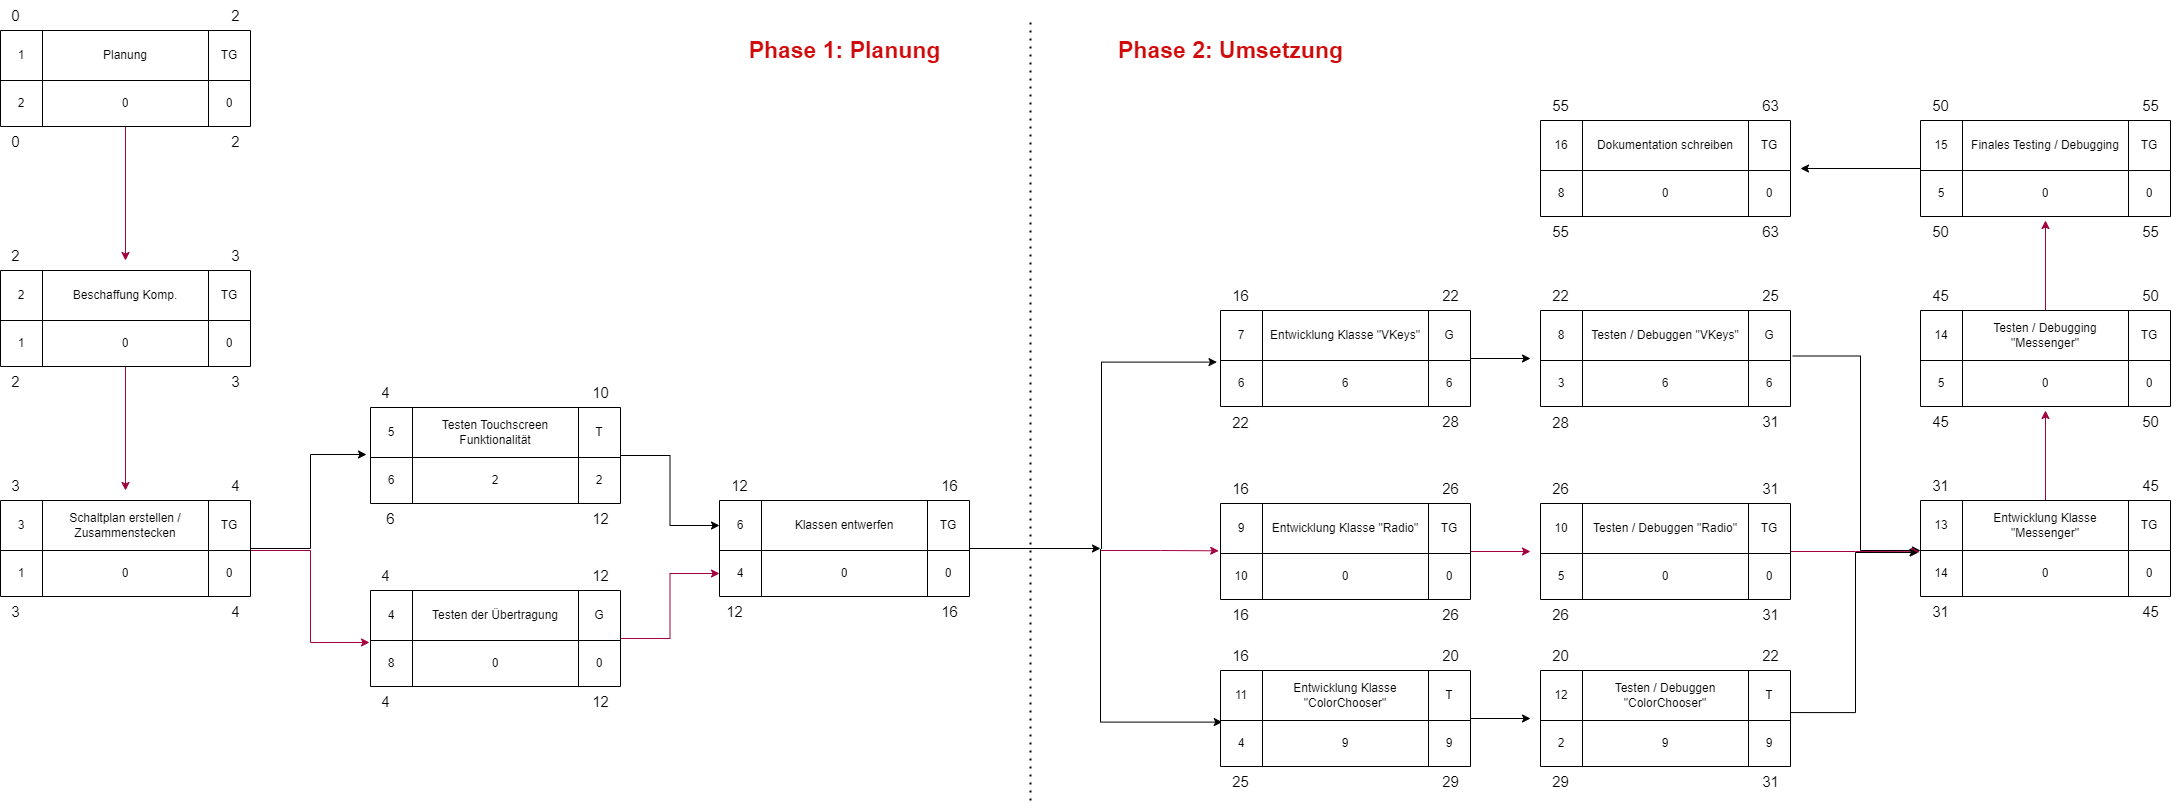
\includegraphics[scale=0.21]{Bilder/Netzplan.png}
        \caption{Netzplan des Projekts}\label{diag:netzplan}
    \end{center}
\end{figure}

\begin{figure}[H]
    \begin{center}
        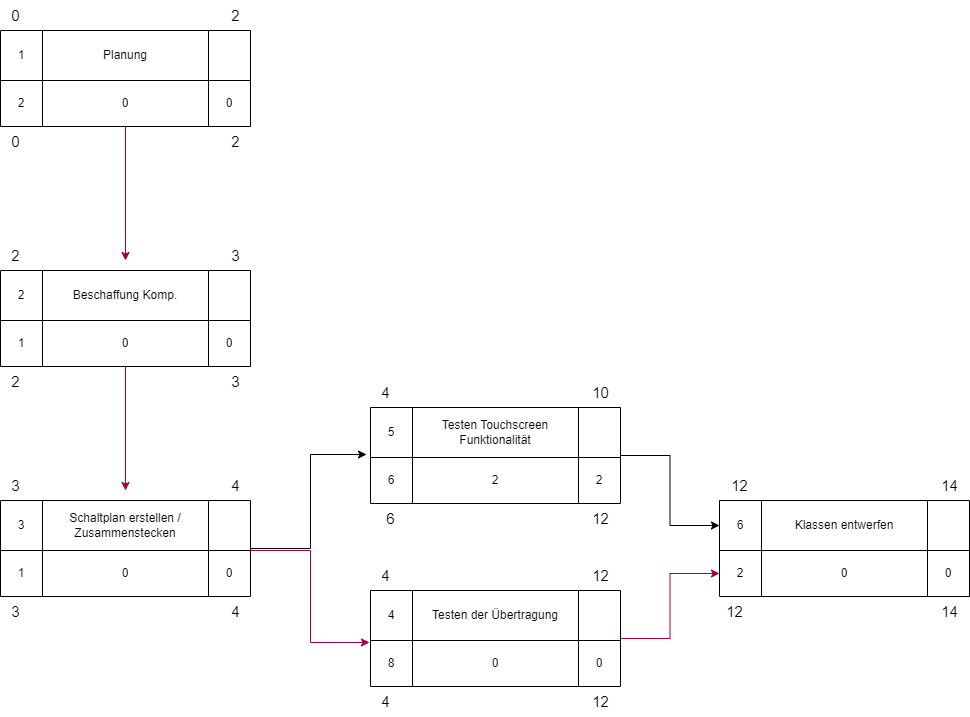
\includegraphics[scale=0.4]{Bilder/netzplan_planung.png}
        \caption{Netzplan der Projektplanung}\label{diag:netzplan_planung}
    \end{center}
\end{figure}

\begin{figure}[H]
    \begin{center}
        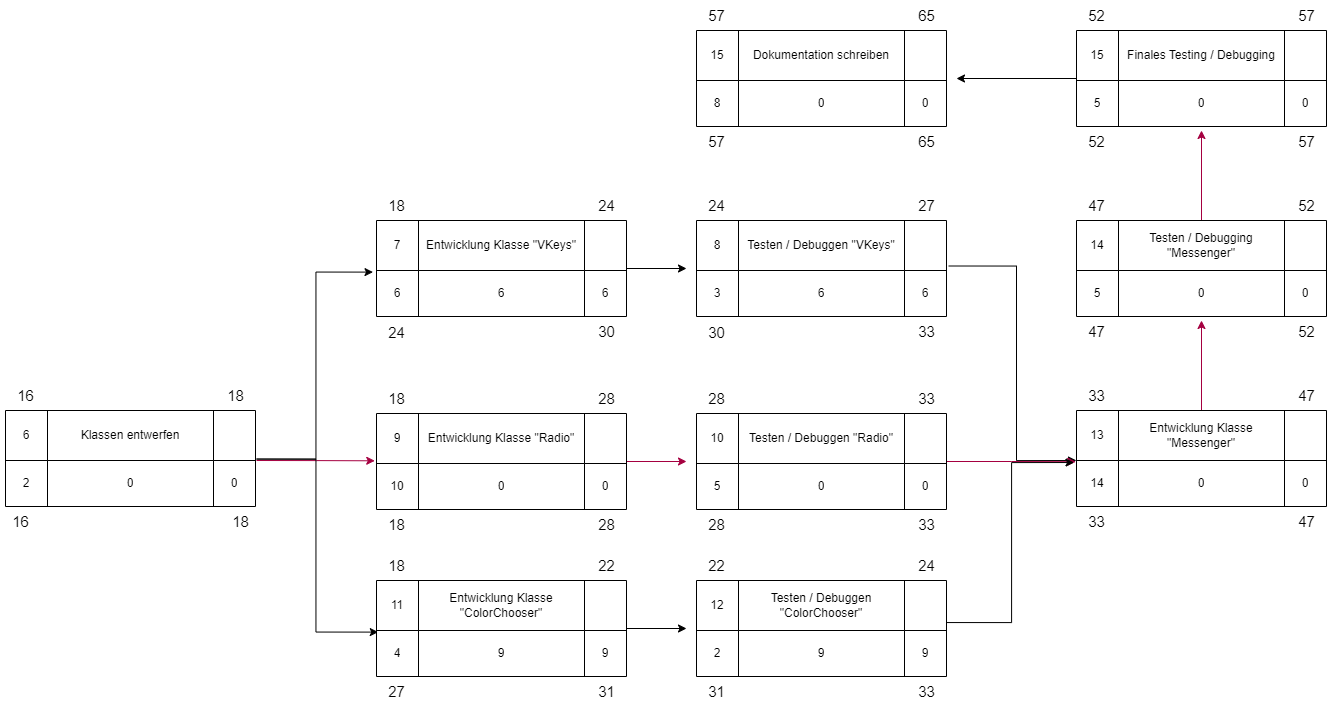
\includegraphics[scale=0.35]{Bilder/netzplan_umsetzung.png}
        \caption{Netzplan der Projektumsetzung}\label{diag:netzplan_umsetzung}
    \end{center}
\end{figure}

\begin{figure}[H]
    \begin{center}
        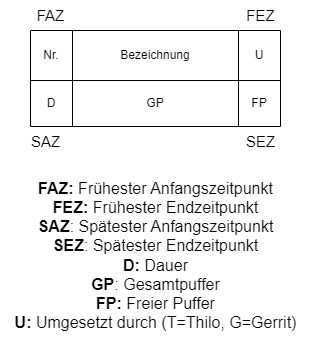
\includegraphics[scale=0.7]{Bilder/netzplan_legende.png}
        \caption{Legende der Netzplan Knoten}\label{diag:netzplan_legende}
    \end{center}
\end{figure}

\begin{figure}[H]
    \begin{center}
        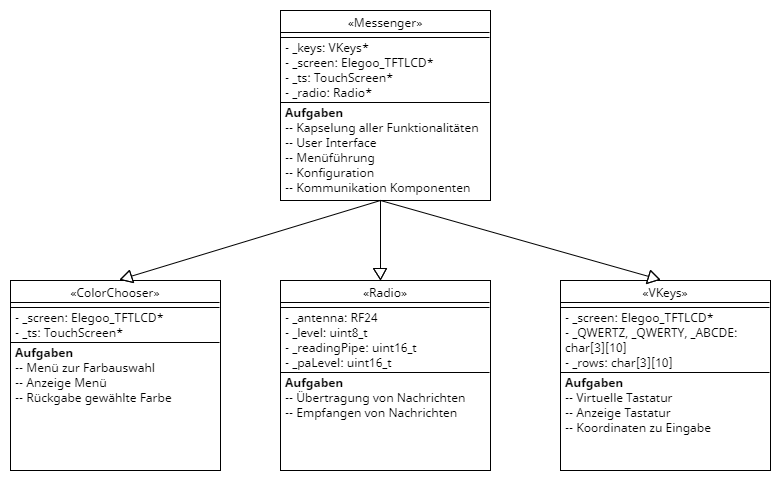
\includegraphics[scale=0.5]{Bilder/Class_Diagram.png}
        \caption{Vereinfachtes Klassendiagramm des Arduino Programms}\label{diag:classdiag}
    \end{center}
\end{figure}

\begin{figure}[H]
    \begin{center}
        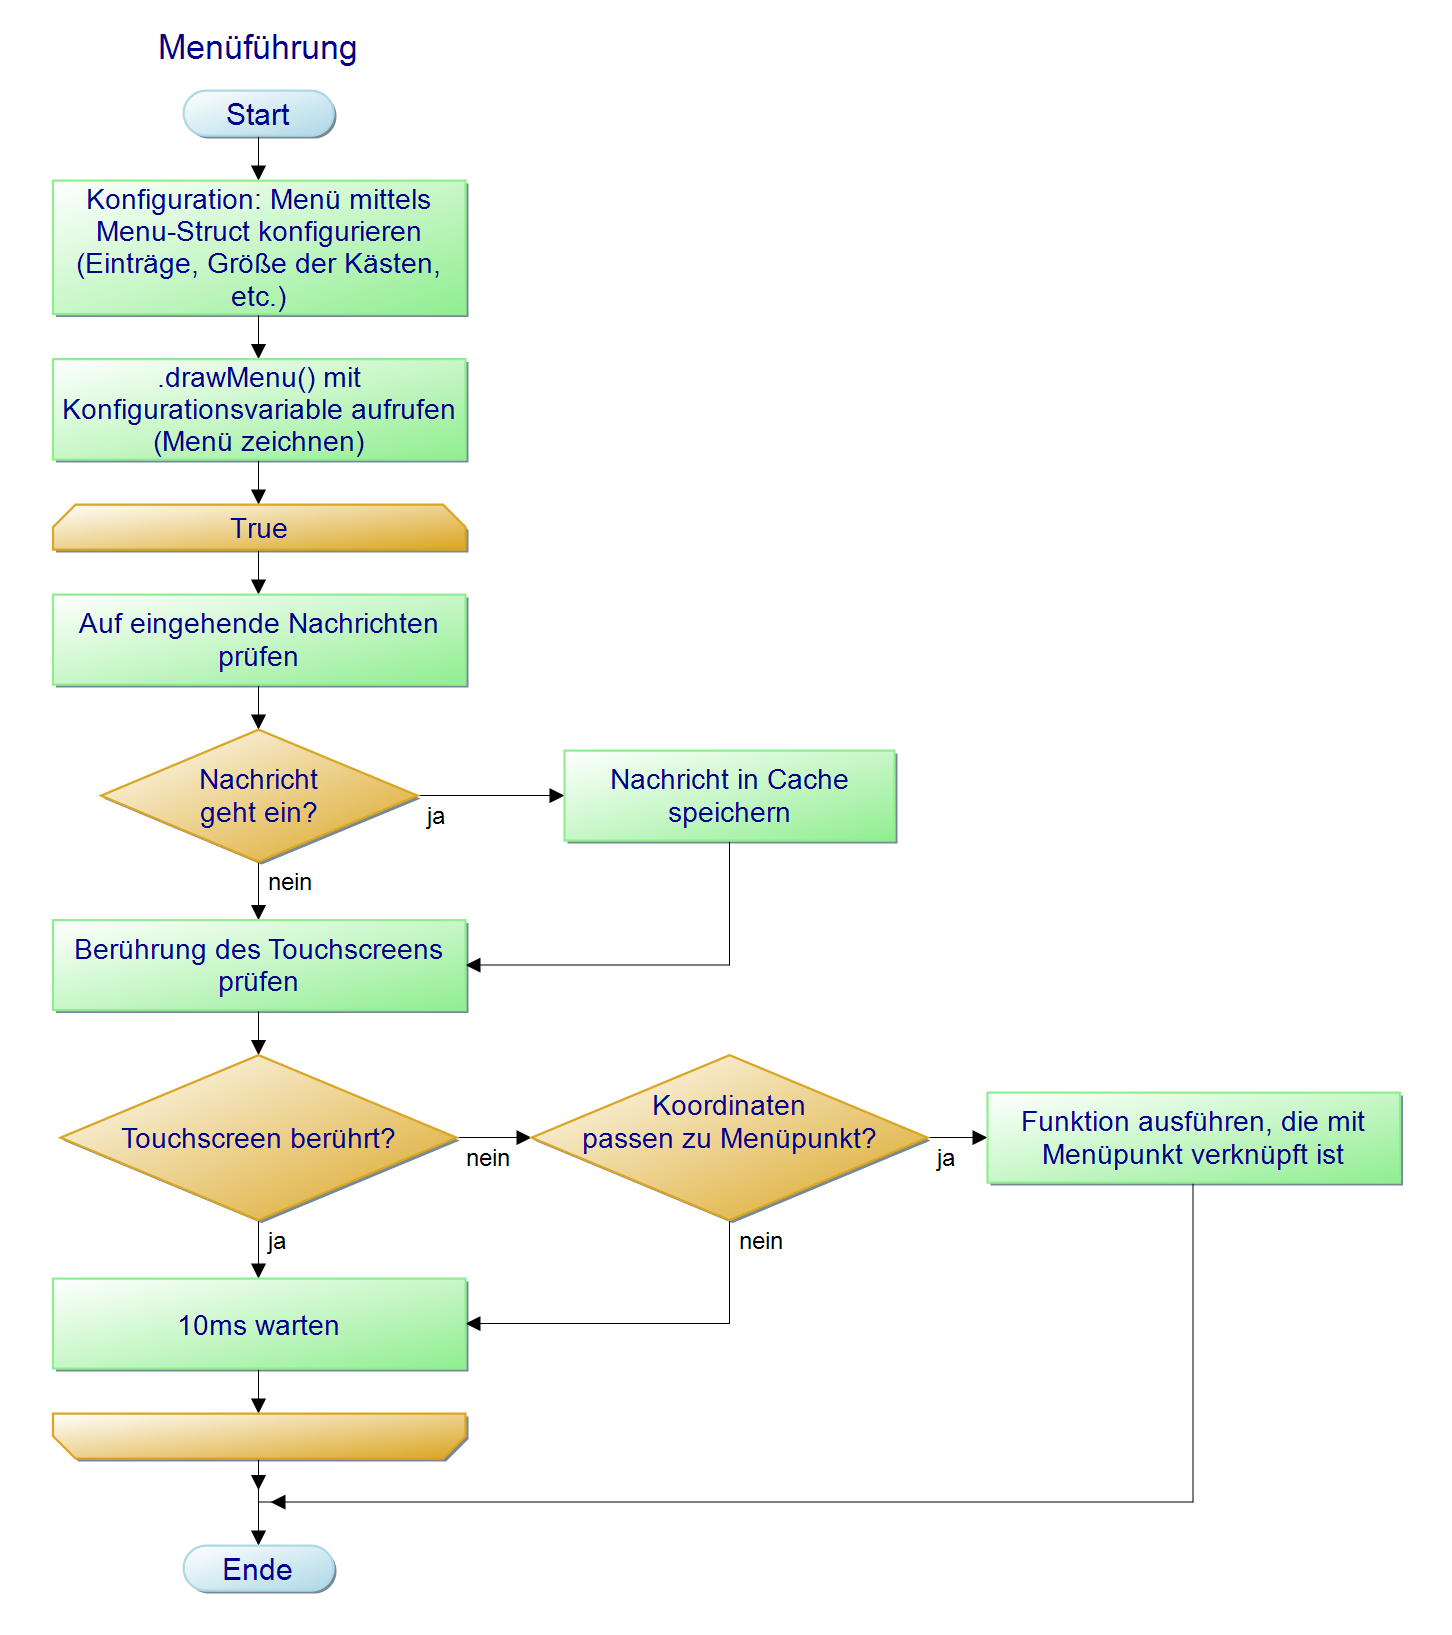
\includegraphics[scale=0.35]{Bilder/Menüführung.png}
        \caption{Aufbau der Menümethoden}\label{diag:menu_pap}
    \end{center}
\end{figure}

\begin{figure}[H]
    \begin{center}
        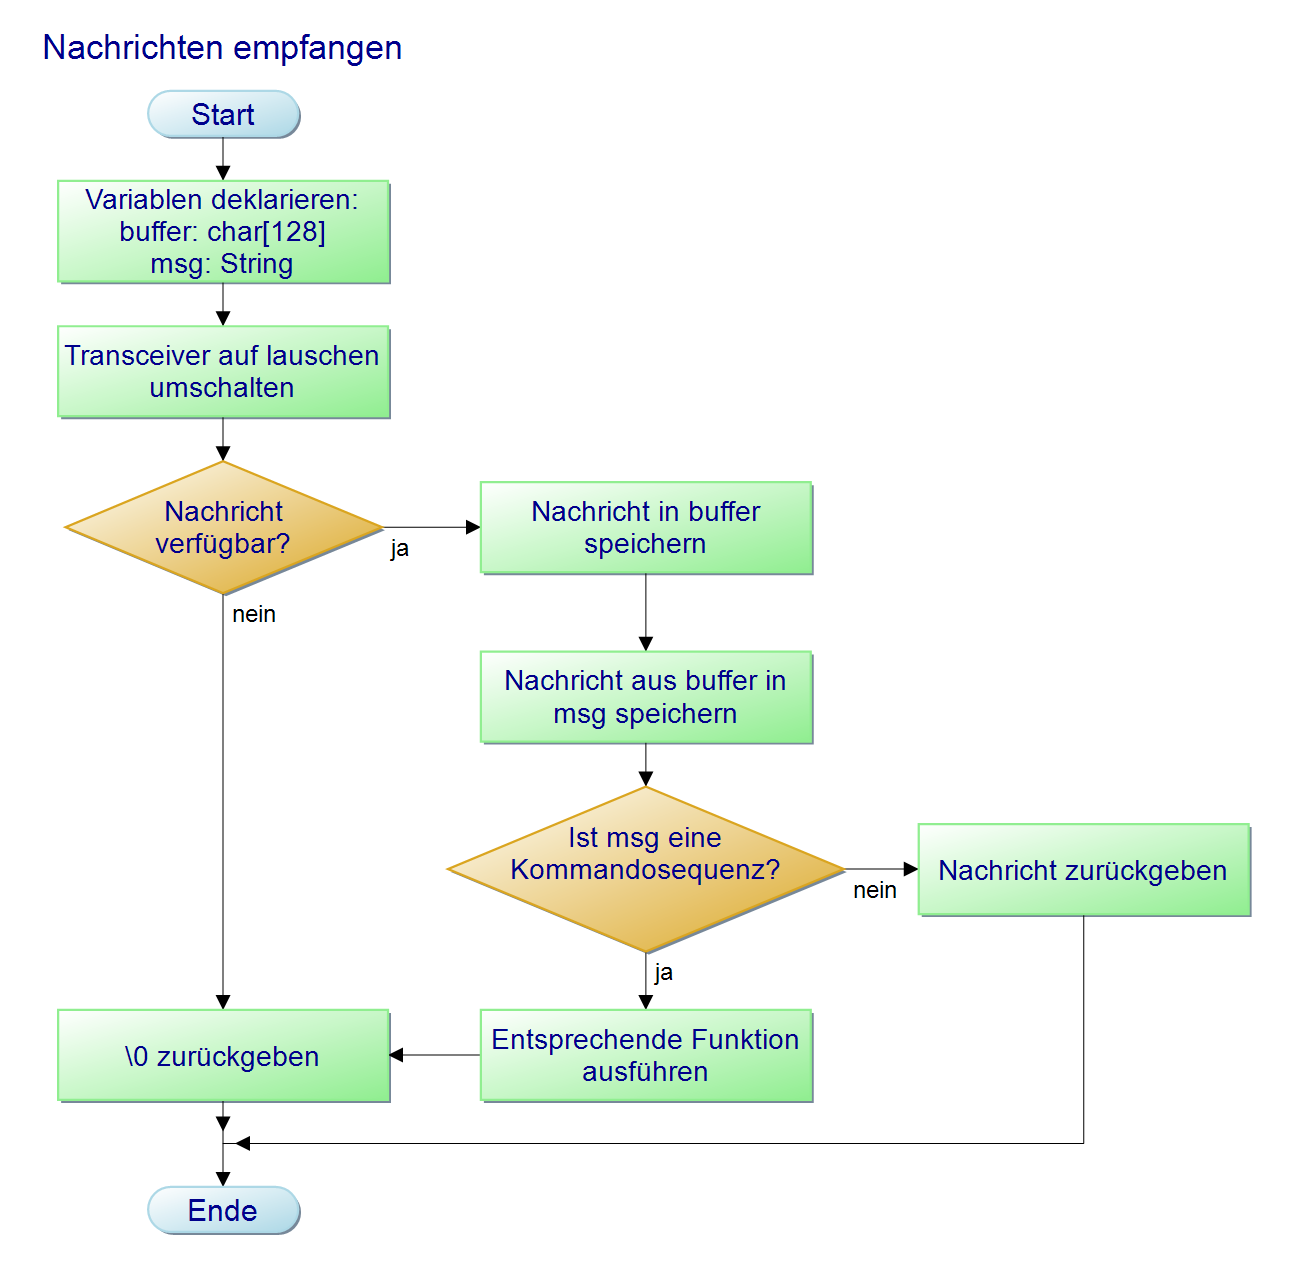
\includegraphics[scale=0.35]{Bilder/Nachrichten_empfangen.png}
        \caption{Ablauf des Nachrichtenempfangs}\label{diag:receive_pap}
    \end{center}
\end{figure}

\begin{figure}[H]
    \begin{center}
        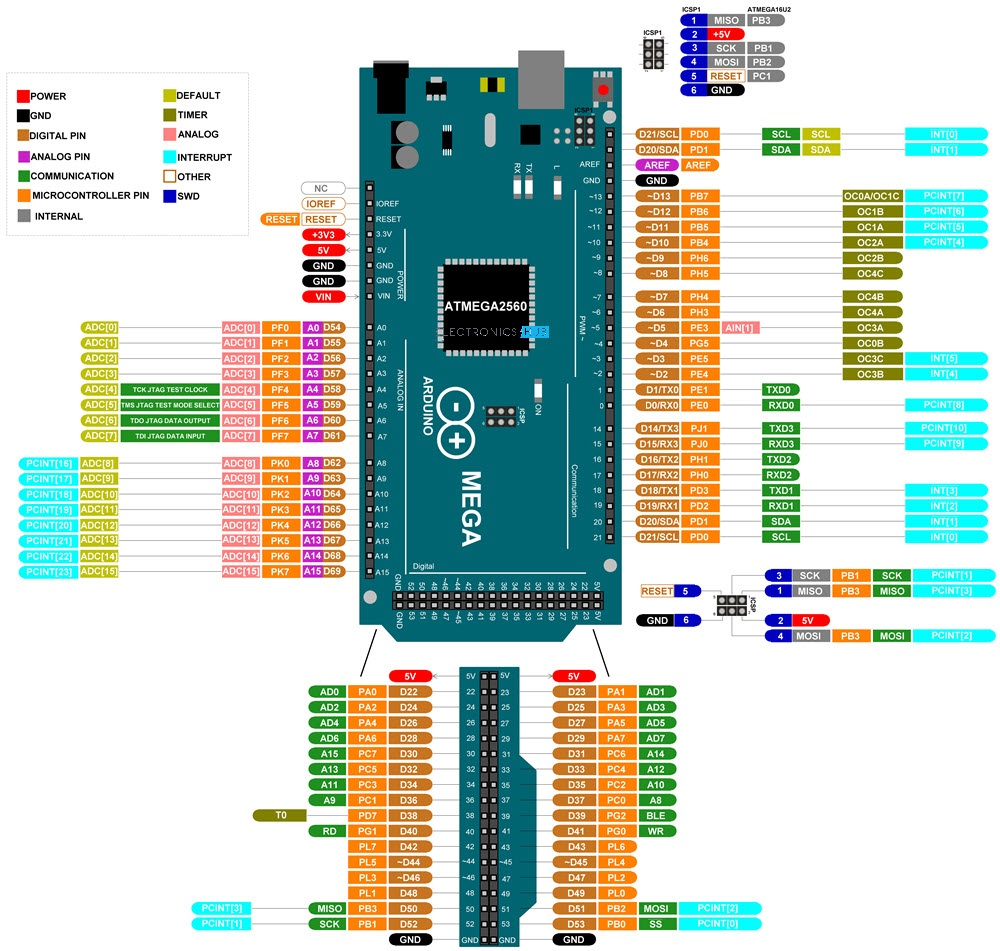
\includegraphics[scale=2.5]{Bilder/Arduino-Mega-Pinout.jpg}
        \caption{Pinout Beschreibung des Arduino Mega 2560 R3, Quelle: Internetquelle~\ref{itm:pinout}}\label{diag:pinout}
    \end{center}
\end{figure}

\begin{figure}[H]
    \begin{center}
        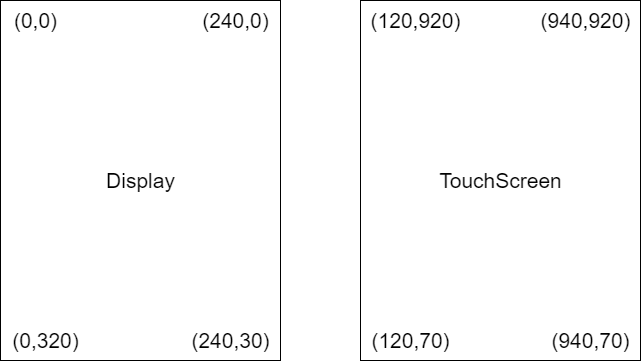
\includegraphics[scale=0.5]{Bilder/touch_grafik_koord.png}
        \caption{Darstellung der Koordinaten von Touchscreen und Display}\label{diag:diskrepanz}
    \end{center}
\end{figure}



\subsection{Bilder}\label{ch:pics}
\begin{figure}[H]
    \begin{center}
        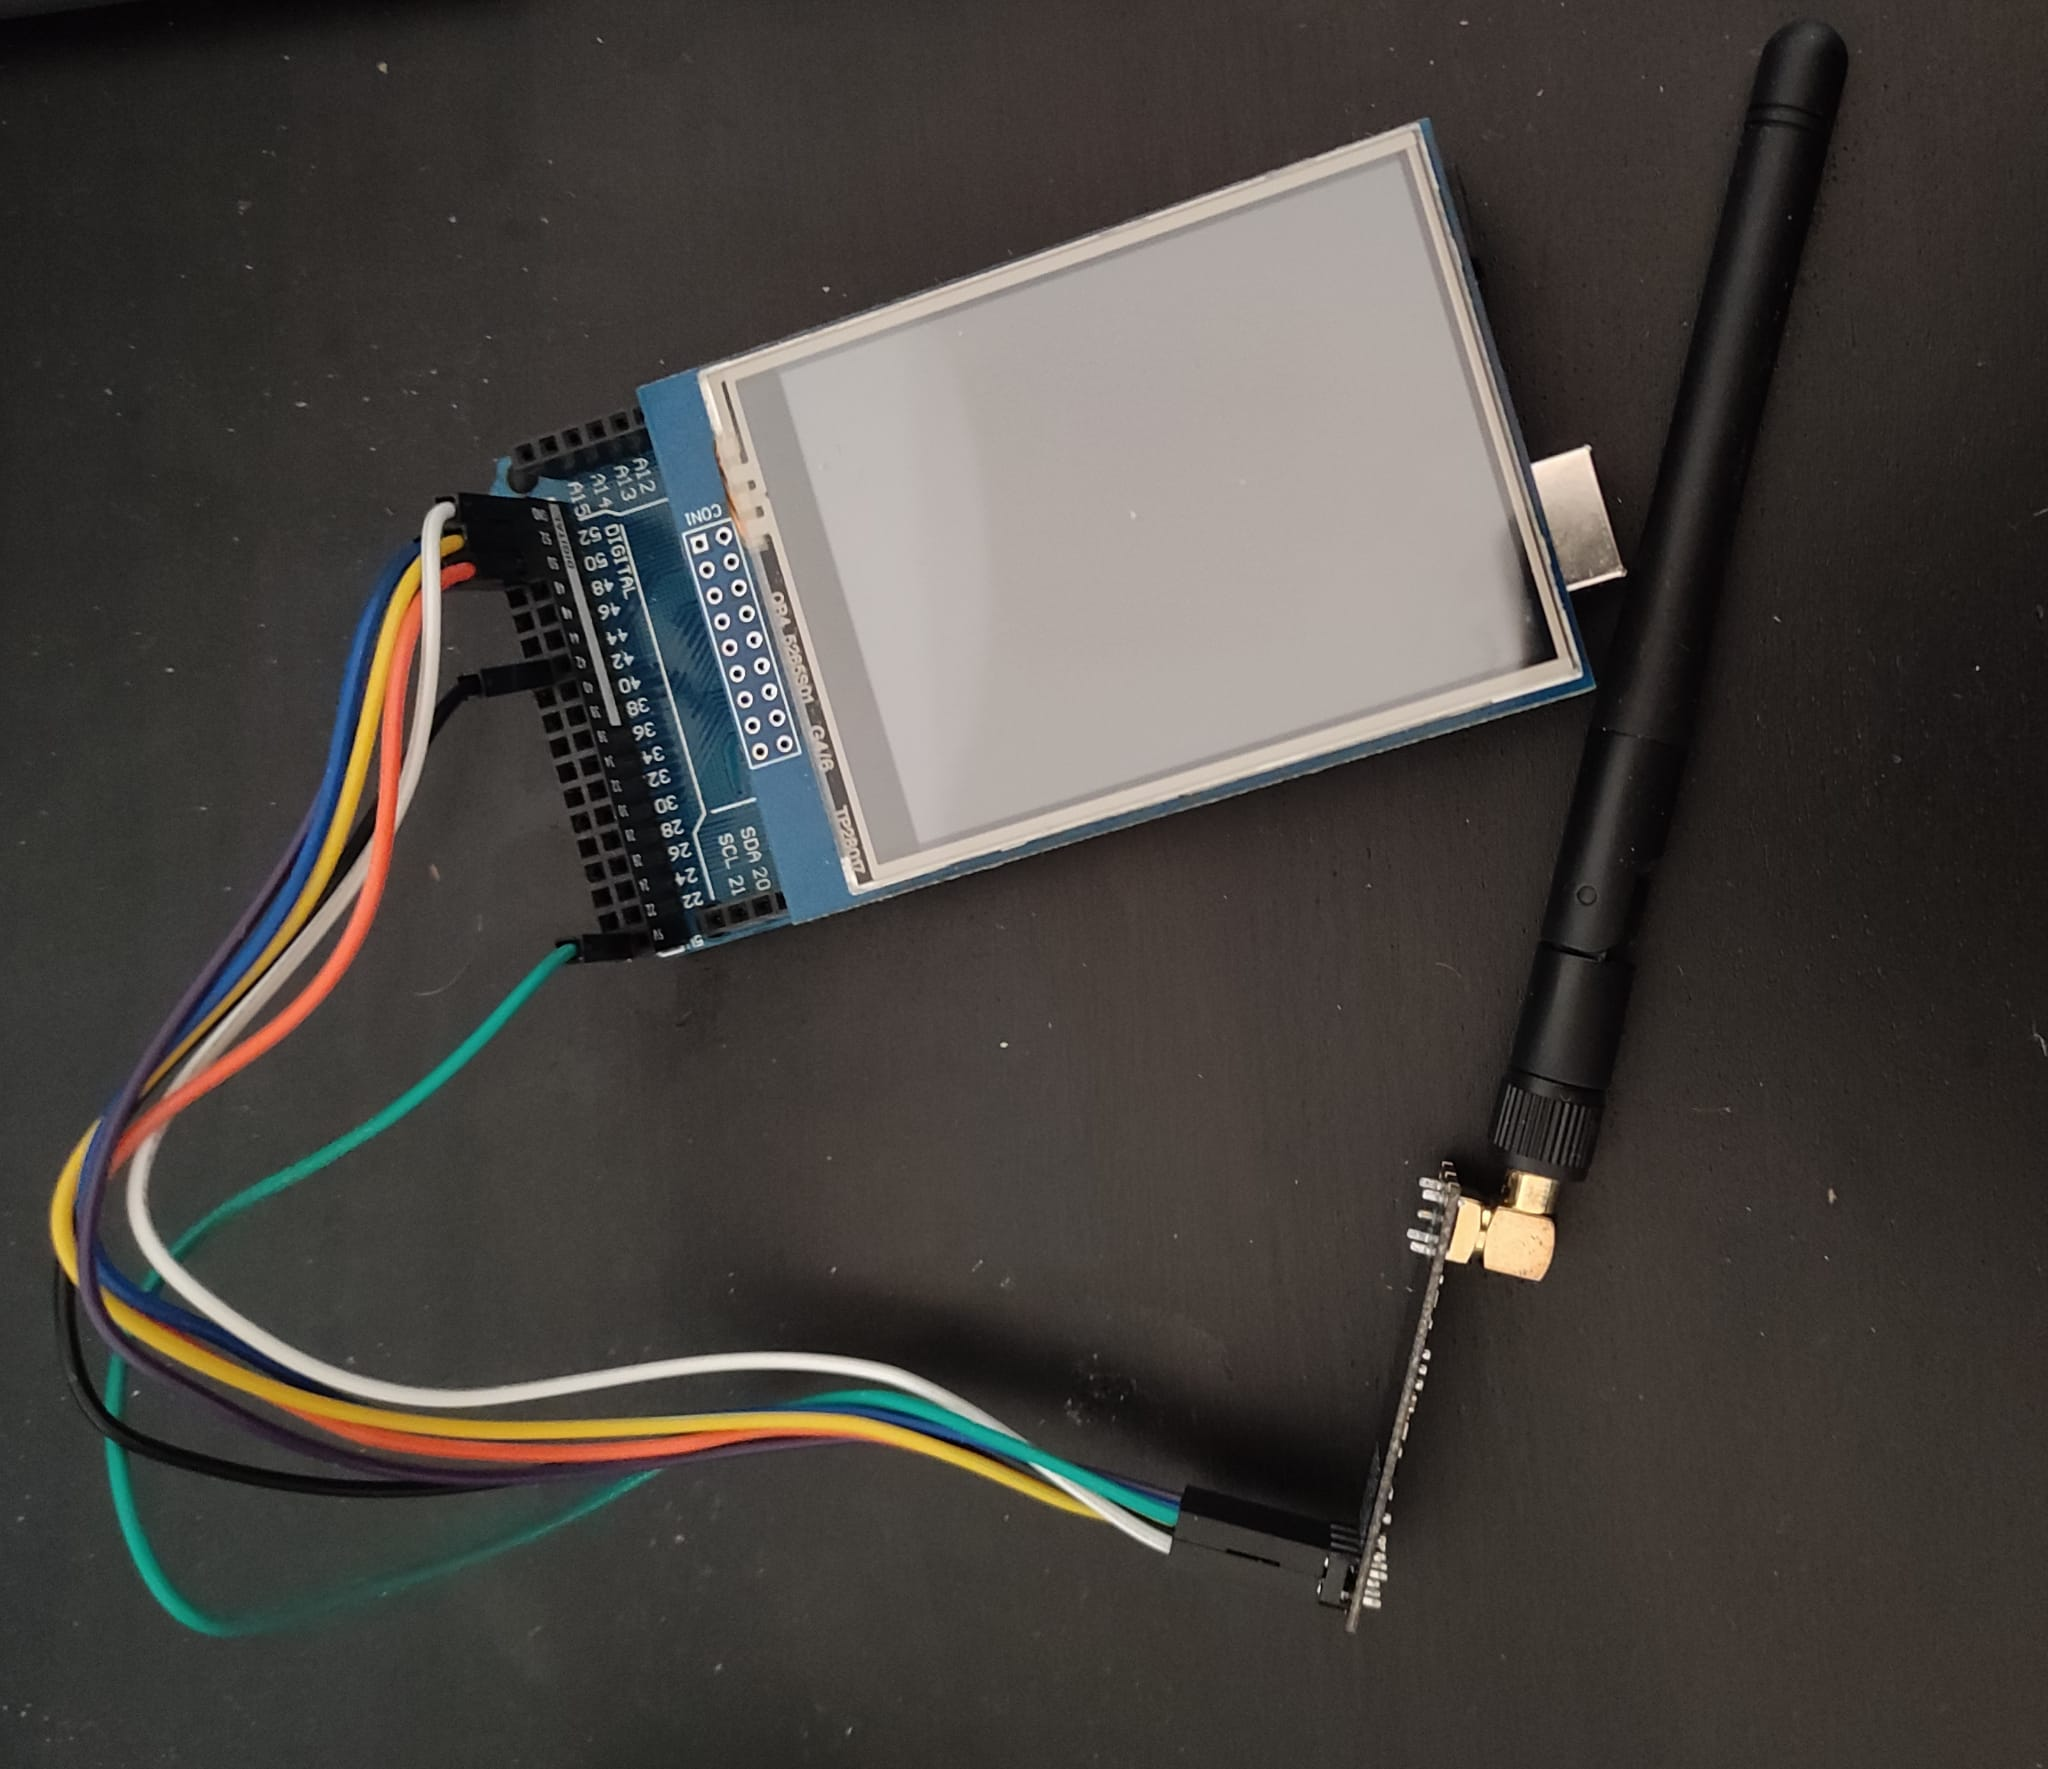
\includegraphics[scale=0.15]{Bilder/projekt_fertig.jpeg}
        \caption{Bild des aufgebauten Projekts}\label{pic:project_done}
    \end{center}
\end{figure}


\newpage
\subsection{Git Repository und Quellcode Auszüge}\label{ch:codeschnipsel}
Das Repository mit dem gesamten Quellcode diesees Projektes befindet sich unter
\\
\url{https://github.com/LeichtMatrosee/TouchPager}
\\
Im Folgenden sind in der Dokumentation benannte Funktionen und Methoden angefügt.

\subsubsection{Klasse: Messenger}
\textbf{Konvertierung Touchscreen zu Screen Koordinaten}\label{code:screenparse}
\begin{lstlisting}
/**
 * @brief 
 * Parses Coordinates from touchpoint to screen coordinates
 * 
 * @param p TSPoint, Point the user touched on display
 * @return ScreenParse Struct containing parsed screen coordinates
 */
ScreenParse Messenger::parseCoords(TSPoint p) {
    ScreenParse parse;
    
    // Touch X: [120,940], Screen X: [0,240]
    // Parse X
    parse.x = (int) ((p.x - 120) / 3.5);

    // Touch Y: [70,920], Screen Y: [0,320]
    // Parse Y
    parse.y = (int) ((p.y - 70) / 2.66);
    return parse;
}
\end{lstlisting}

\begin{flushleft}\textbf{Beispiel Menüführung: Optionenmenü}\end{flushleft}
\begin{lstlisting}
/**
 * @brief 
 * Options menu
 * 
 */
void Messenger::optsMenu(void) {
    pinMode(A2, OUTPUT);
    pinMode(A3, OUTPUT);
    Menu menu;
    menu.menuStart = 60;
    menu.menuThickness = 40;
    menu.menuOffset = 20;
    menu.header = "Optionen";
    menu.entries[0] = String("Farben");
    menu.entries[1] = String("Tastatur");
    menu.entries[2] = String("Distanz");
    menu.entries[3] = String("Zurueck");
    menu.entries[4] = String("\0");

    drawMenu(menu);
    delay(100);

    while (true) {
        String inc = receiveMessage();
        if (inc != "\0") Serial.println(inc);
        int selection = -1;
        
        // Get touchpoint
        digitalWrite(13, HIGH);
        TSPoint p = _ts->getPoint();
        digitalWrite(13, LOW);

        // If touch was recognized
        if (p.z > _minTouch) {
            // Get selected menu poin
            selection = getSelection(menu.menuStart, menu.menuThickness, menu.menuOffset, 4, parseCoords(p));

            Serial.println("Selection: " + String(selection));
            
            switch (selection) {
                case -1: break;
                case 1: colorMenu(); return;
                case 2: keysMenu(); return;
                case 3: distanceMenu(); return;
                case 4: return;
                default: break;
            }
        }
        delay(10);
    }

    Serial.println("Returning from optsMenu");
}
\end{lstlisting}

\subsubsection{Klasse: Radio}
\textbf{Empfangen von Nachrichten}\label{code:receive}
\begin{lstlisting}
/**
 * @brief 
 * Receives message from radio frequency
 * 
 * @return String received message or \0, if nothing was gotten
 */
String Radio::receiveMessage(void) {
    char buffer[128] = "";
    String msg = "";

    // Switch from sending to listening
    if (!_listening) switchState();

    // If no message is available, return universal break character
    if (!_antenna.available()) return "\0";
    Serial.println("Receiving: Antenna available");

    // Read available payload
    _antenna.read(&buffer, sizeof(buffer));

    // Convert payload (char array) to string for easier handling
    for (int i = 0; i < 128; i++) {
        msg += String(buffer[i]);
        if (buffer[i] == '\0') break;
    }

    Serial.println("Receiving: Received char Array: " + msg);

    return msg;
}
\end{lstlisting}

\begin{flushleft}\textbf{Senden von Nachrichten}\label{code:sending}\end{flushleft}
\begin{lstlisting}
/**
* @brief 
* Sends message given in param
* 
* @param msg Message to be sent
* @return true If sending was successful
* @return false otherwise
*/
bool Radio::sendMessage(String msg) {
    String sendTest = "";
    bool tx_ok, tx_fail, rx_ready, test = true;
    char buffer[128];
    msg.toCharArray(buffer, msg.length() + 1);
    
    Serial.println("Sending message: " + msg);
    Serial.println("Listening State: " + String((_listening ? "listening" : "writing")));

    if (_listening) switchState();
    
    Serial.println("Listening State: " + String((_listening ? "listening" : "writing")));

    // convertStringToCharArray(msg, buffer);
    for (int i = 0; i < msg.length(); i++) {
        sendTest += String(buffer[i]);
    }
    Serial.println("Sending: Char Arr after conversion: " + sendTest);
    
    test = _antenna.write(&buffer, sizeof(buffer));

    if (!test) {
        Serial.println("Sending unseccessful");
        _antenna.whatHappened(tx_ok, tx_fail, rx_ready);
        Serial.println("OK: " + String((tx_ok ? "Yes" : "No")) + ", FAIL: " + String((tx_fail ? "Yes" : "No")) + ", READY: " + String((rx_ready ? "Yes" : "No")));
        switchState();
        return false;
    }

    Serial.println("Returning from sending");
    switchState();
    return true;
}
\end{lstlisting}

\begin{flushleft}\textbf{Konvertierung String zu Char-Array}\label{code:transpose_s_to_arr}\end{flushleft}
\begin{lstlisting}
/**
 * @brief
 * Converts a given String s to a char array and saves it to given pointer a
 * 
 * @param s Strung to be converted to char array
 * @param a Pointer to char array
 */
void Radio::convertStringToCharArray(String s, char a[128]) {
    int counter = 0;

    // Iterate through entire String and add character to char array
    for (int i = 0; i < s.length(); i++) {
        a[i] = s.charAt(i);
        counter++;
    }

    // Fill up char array with empty values
    for (int i = counter; i < 128; i++) {
        a[i] = '\0';
    }

    Serial.println("Char Arr after conversion: " + String(a));
}
\end{lstlisting}

\begin{flushleft}\textbf{Wechsel zwischen senden und lauschen}\label{code:switch}\end{flushleft}
\begin{lstlisting}
/**
 * @brief 
 * Switches from listening to sending and the other way around
 * 
 */
void Radio::switchState() {
    byte _adress[6] = "00001";
    // Invert listening
    _listening = !_listening;

    // If listening: Prepare antenna for listening. Otherwise: Prepare antenna for sending
    if (_listening) {
        _antenna.openReadingPipe(_readingPipe, _adress);
        _antenna.startListening();
    } else {
        _antenna.stopListening();
        _antenna.openWritingPipe(_adress);
    }

    _antenna.setPALevel(_level);
}
\end{lstlisting}

\subsubsection{Klasse: VKeys}
\begin{flushleft}
    \textbf{Erkennung Tastatur Knopf}\label{code:keys}
\end{flushleft}
\begin{lstlisting}
/**
 * @brief 
 * Returns selected char by calculating, which column and row was pressed from passed x and y coords
 * 
 * @param x X coordinate from touchscreen selection
 * @param y Y coordinate from touchscreen selection
 * @return String Selected character parsed to a string, BACK if back button was selected and DONE, if done button was selected
 */
String VKeys::getCharFromCoords(int16_t x, int16_t y) {
    int row, column;

    // Complete Y: [70,920], range 850, keyboard [70,475], keyboard range of 405, 4 rows so 405/4 = 101.25
    if (y > 475) return String('\0');
    row = (int) ((y - 70)/ 101.25);

    // row 0 is spacebar, therefore return escaped space immediately, as nothing else is there.
    if (row == 0) {
        int tempX = (int)((x - 120) / 3.5);

        if (tempX < (_screen->width() / 4)) {
            return String("BACK");
        } else if (tempX > 3*(_screen->width() / 4)) {
            return String("DONE");
        }
        return String(" ");
    }

    if (row > 3) return String('2');

    // X Range ca. 120 - 920 for 10 columns, therefore 800 / 10 = 80
    column = (int) ((x - 120)/ 80);

    if (column < 11 && column >= 0 && row < 4 && row >0) return String(_special ? _specialChars[(3-row)][column] : _rows[(3-row)][column]);
    
    return String('-');
}
\end{lstlisting}

\subsubsection{Klasse: ColorChooser}
\begin{flushleft}\textbf{Erkennen der ausgewählten Farbe}\label{code:color}\end{flushleft}
\begin{lstlisting}
/**
 * @brief 
 * Analyses coordinates passed into function and returns selected color
 * 
 * @param coords Coordinates of touchpoint, parsed to screen coordinates
 * @return uint16_t chosen Color or 0, if cancelled or -2, if selection was not valid
 */
uint16_t ColorChooser::getSelection(Coords coords) {
    int column, row;

    Serial.println("CC: X: " + String(coords.x) + ", Y: " + String(coords.y));

    // Check, if touchpoint is at height of cancel button
    if (320 - coords.y > 250) return 0;

    // If coordinates are out of valid ranges, return failure marker
    if (coords.x < 35 || coords.x > 215) return -2;
    if (coords.x < 135 && coords.x > 100) return -2;

    // If x is less than 100, it has to be first column (index 0), otherwise second column (index 1)
    column = coords.x < 100 ? 0 : 1;

    // Invert coordinates (320-y, because screen is 320 high) and divide by 60, because that's the 
    // height of the boxes, to get the row
    row = (int)((320 - coords.y) / 60);

    // Variable basically only exists, so that we don't try to reach indices the array does not have
    // This works, because the first column has indices 0,2,4,6 and second has 1,3,5,7
    int safeHandler = column + (row*2);

    // If selection > 7, set selection to failure, otherwise set selection to selected color
    uint16_t selection = (safeHandler > 7 ? -2 : _colors[safeHandler]);

    return selection;
}
\end{lstlisting}











\end{small}
\newpage
\section{Glossar}
\subsection{Technische Begriffe}
\textbf{Multithreading\label{def:multithreading}}
\\
Unter Multithreading versteht man in der Informatik den Prozess, ein Programm in mehrere Teilstränge aufzuteilen, die parallel 
ausgeführt werden.\footnote{Vgl. Internetquelle~\ref{itm:multithread}}
\\
\\
\textbf{SPI-Bus\label{def:SPI}}
\\
SPI steht für Serial Peripheral Interface und ist ein, aus drei Leitungen bestehendes, Bussystem nach dem Master-Slave Prinzip, mit dem die Kommunikation
verschiedener Komponenten gesteuert werden kann.\footnote{Vgl. Internetquelle~\ref{itm:SPI}}
\subsection{Arduino Begriffe}
\textbf{Shield\label{def:shield}}
\\
Ein Shield ist ein Schaltplatte, die die Funtkionalität eines Arduinos erweitern kann und meistens so konzeptioniert ist, dass sie direkt in den Arduino gesteckt werden kann und diesen somit
zum Teil oder vollständig abdeckt.\footnote{Vgl. Internetquelle~\ref{itm:shield}}
\newpage
\section{Quellenverzeichnis}
\subsection{Internetquellen}
\begin{enumerate}
    \item Storage Insider: Was ist Multithreading - Online unter \url{https://www.storage-insider.de/was-ist-multithreading-a-1017586/} $\left[\text{07.01.2023}\right]$ \label{itm:multithread}
    \item Computer Hope: Arduino Shield - Online unter \url{} $\left[\text{07.01.2023}\right]$ \label{itm:shield}
    \item Mikrocontroller.net: Serial Peripheral Interface - Online unter \url{https://www.mikrocontroller.net/articles/Serial_Peripheral_Interface} $\left[\text{15.01.2023}\right]$ \label{itm:SPI}
    \item Electronics Hub: Arduino Mega Pinout - Online unter \url{https://www.electronicshub.org/wp-content/uploads/2021/01/Arduino-Mega-Pinout.jpg} $\left[\text{15.01.2023}\right]$ \label{itm:pinout}
\end{enumerate}

\subsection{Links genutzter Hardware}\label{ch:hardwarelinks}
\begin{enumerate}
    \item nRF24L01+ Transceiver: \url{}\label{itm:transceiverlink}
    \item Elegoo Arduino Mega R3: \url{}\label{itm:arduinolink}
    \item Elegoo TFT Touchscreen: \url{}\label{itm:tftlink}
\end{enumerate}

\subsection{Links genutzter Software}\label{ch:softwarelinks}
\begin{enumerate}
    \item RF24: Online unter \url{https://github.com/nRF24/RF24}\label{link:rf24}
\end{enumerate}

\end{document}